\chapter{Data stores}
\label{ch:data-stores}

\section{Selected data stores}
\label{sec:selected-data-stores}

% TODO: reference for large number
Due to the large number of active and maintained NoSQL data stores it is not feasible to consider all of them for this research.
We will consider every NoSQL category, discuss the use of the respective categories applied to the use case, and decide whether or not it will be included in the research.
In the applicable NoSQL categories the most popular data stores are selected, where popularity is based on certain predetermined parameters.

\textcite{DBEngine2018} maintains a list of database systems ranked by popularity, based on parameters such as number of mentions on websites, Google Trends and relevance in social networks.
% TODO: reference for LinkedIn and Upwork
These parameters are also cross-referenced with professional networks such as LinkedIn and Upwork using the number of available job offers and professional profiles.
This ranking is called the DB-Engine Ranking.
The list includes not only NoSQL databases but also other types of data storage systems such as relational database systems.

% TODO: reference for Gartner
The information technology division of Gartner maintains a yearly report on emerging relational and non-relational database technologies.
% TODO: elaborate

The DB-Engine Ranking is used primarily to determine which data stores are the most interesting to consider in this research.
The Magic Quadrant for Operational Database Management Systems was used as a secondary resource.
Due to licensing concerns regarding the Open Webslides project, database systems that do not fall under a free license as classified by the \textcite{FreeSoftwareFoundation1985} will not be considered.

% TODO: references
Certain categories of NoSQL data stores will not be considered.
Key-value stores will not be accounted for due to the relative simplicity of this type of data store.
The main use case of key/value stores is not storing more complex information, rather the emphasis lies more on scalability and consistency.
Processing complex queries that consist of the NoSQL equivalent of relational joins is not efficient in key-value data stores.
Implementing the proposed data model and queries in such a system is a more ambitious task that does not lie within the scope of the research.

Column-oriented data stores are a category of NoSQL data stores that is questionably useful in this case study.
% TODO: reference
These data stores are commonly seen as inverse relational database systems, where the storage of attributes per entity is more flexible regarding nullable values and unstructured information.
Column-oriented data stores are very efficient when retrieving a subset of columns for a certain record.
Since the data store will be deployed as additional data store next to the authoritative relational database, it will not contain any data that will not be used when querying the database.
This workflow cancels out the efficiency and usefulness of column-oriented data stores, and subsequently we will not consider this NoSQL category as a viable candidate.

Furthermore, comparison and application of NewSQL data stores will not be included in this paper either.
As described in \cref{ch:overview}, NewSQL aims to provide scalable performance similar to that of NoSQL while still guaranteeing ACID properties.
Since ACID is not a major concern for this use case, NewSQL does not provide significant advantage over NoSQL, and will therefore be omitted from the comparison.
Similarly, object-oriented and multi-model database such as OrientDB \autocite{OrientDB2010} are not within scope of this research.

In conclusion, document and graph data stores will provide the most beneficial data storage and are the main focus of this research.\\

The most popular document database systems according to the DB-Engine Ranking are MongoDB \autocite{MongoDB2009}, CouchDB \autocite{CouchDB2005} and Couchbase \autocite{Couchbase2010}.
While Couchbase is technically a multi-model data store, it is being ranked as a document database.
However, Couchbase is a conceptual merge between CouchDB and Membase, and mainly adds improved scalability, clustering and auto-sharding.
Couchbase will not be investigated upon in a practical capacity, however it is considered as an option to increase multi-host scalability.
This leads to MongoDB and CouchDB being the contestants in the document database system category.

Finally, as sole graph database the Neo4j system \autocite{Neo4j2007} stands out greatly over competitors in the ranking.
This database system will be analyzed as only graph database in this research.

In conclusion, the data stores included in the study will be MongoDB and CouchDB as document databases, and Neo4j as graph databases.

\section{Comparative study}
\label{sec:comparative-study}

Data stores and databases can be compared and analyzed using many quantitative and qualitative aspects.
In this section we propose a selection of criteria based on the usefulness applied to the studied use case.
Since the landscape and feature-set of NoSQL data stores is changing on a weekly base, the impact of these technologies must be carefully considered in order to reach a durable conclusion in this research.

The features of a data store that are taken into account in this comparative study are:

\begin{itemize}
  %% Features
  \item Querying capabilities
    \begin{itemize}
      \item Language
      \item Protocol
      \item MapReduce
    \end{itemize}

  %% Language
  \item Programming language
  \item Language bindings

  %% Integrity
  \item Integrity model
  \item Atomicity
  \item Revision control
  \item Consistency

  %% Scalability
  \item Persistence
  \item Partitioning
  \item High Availability
  \item Concurrency
  \item Replication

  %% Various
  \item License
  \item Commercial support
\end{itemize}

Certain aspects are not relevant to the presented use case because of various reasons.
Aspects omitted from the study are:

\begin{itemize}
  \item Security
  \item Compression
  \item Full-text search
  \item Geospatial functionality
  \item Cloud hosting
\end{itemize}

%% Omitted aspects
The specific use case described in this thesis does not focus on security, since the data store is not public facing and clients do not interact directly with it.
Security measures include but are not limited to authentication, authorization, encryption and auditing.
None of these are features that are required or useful for the comparison.
Authentication and authorization is functionality that is present in all databases.
It introduces the concept of multiple clients or roles connecting to a database, and assigning permissions to these clients in order to enforce permissions-based access.
However since there will only be one client connecting to the database - the platform itself - deeper integration with LDAP, ActiveDirectory or similar is superfluous and omitted from the comparison.

Encryption refers to the mechanism where data is encrypted and unreadable for unauthorized third parties.
Encryption in databases is threefold: encryption of data at rest, client-to-server communication and server-to-server communication \autocite{Grolinger2013}.
However, since data protection is a comprehensive topic, it does not fall within the scope of this research.
Consequently, encryption functionality is not considered in the comparative study.

Database auditing is a facility offered by the database management system that keeps track of the usage of database resources and authorization.
Operations on the database leave a trail of events, called an \textit{audit log}.
Similarly to authentication, the usefulness of this functionality is somewhat lost when there is only one client operating on the database.
However, many security standards such as PCI-DSS and HIPAA require the existance of an audit log.

Compression of data in the database is not included in the comparison.
Builtin compression may provide additional storage space but as it is a disk space-CPU usage tradeoff we have chosen to only consider CPU usage.
Akin to compression, we leave the choice of cloud hosting up to the database administrator.

Full-text search and geospatial functions are provided by certain data stores, however these features are not used by the platform and subsequently are not relevant to this comparative study.\\

%% Comparative study

\begin{landscape}
  % TODO: references
\begin{table}
  \sffamily
  \begin{tabular}{l l l l l l l l l}
    \toprule
    &
    &
    \multicolumn{3}{l}{\textbf{Querying}} &
    \multicolumn{2}{l}{\textbf{Language}} &
    & \\

    \cline{3-7}

    &
    &
    \textbf{Language} &
    \textbf{Protocols} &
    \textbf{MapReduce} &
    \textbf{Language} &
    \textbf{Language bindings} \\

    \cline{3-8}

    \multirow{2}{*}{\makecell[l]{\textbf{Document}\\\textbf{stores}}} &
    \textbf{MongoDB} &
    \small{JavaScript} &
    \makecell[l]{MongoDB Wire Protocol\\REST \footnotemark[1]} &
    Yes &
    C++ &
    % https://docs.mongodb.com/manual/applications/drivers/
    \makecell[l]{C/C++, C\#, Java,\\Node.js, Perl, PHP,\\Python, Ruby, Scala\\Erlang\footnotemark[1], Go\footnotemark[1]} \\

    \cline{2-8}

    &
    \textbf{CouchDB} &
    REST &
    HTTP &
    Yes &
    Erlang &
    % https://cwiki.apache.org/confluence/display/COUCHDB/CouchDB+clients
    \makecell[l]{C/C++\footnotemark[1], Dart\footnotemark[1], Go\footnotemark[1],\\Java\footnotemark[1], Lua\footnotemark[1], Node.js\footnotemark[1],\\Python\footnotemark[1], R\footnotemark[1],\\Ruby\footnotemark[1], Scala\footnotemark[1]} \\

    \cline{2-8}

    \makecell[l]{\textbf{Graph}\\\textbf{stores}} &
    \textbf{Neo4j} &
    \makecell[l]{Cypher\\SparQL\footnotemark[1]\\Gremlin\footnotemark[1]} &
    \makecell[l]{HTTP\\Bolt} &
    No &
    Java &
    % https://neo4j.com/docs/developer-manual/current/drivers/
    \makecell[l]{C\#, Java,\\JavaScript, Python,\\C/C++\footnotemark[1], Clojure\footnotemark[1],\\Erlang\footnotemark[1], Go\footnotemark[1], Haskell\footnotemark[1],\\Perl\footnotemark[1], PHP\footnotemark[1], R\footnotemark[1], Ruby\footnotemark[1]} \\

    \bottomrule
  \end{tabular}

  \caption{NoSQL data stores: Querying and language support}
  \label{tbl:query-language}
\end{table}

\footnotetext[1]{3\textsuperscript{rd} party community supported}

\end{landscape}

One of the most important factors when deciding on a NoSQL data store is the capability to communicate with the data store, since NoSQL does not have a unified interface like SQL signifies for relational databases.
Choosing a certain data store may allow the developer to integrate data storage easier into the application.
Every NoSQL data store has its own standard for composing queries, related but not depending on the protocol used for communication with the server.
MongoDB allows querying using a JavaScript API, natively over MongoDB's binary protocol or over HTTP (REST) using a third party plugin.
% TODO: reference
Subsequently, MongoDB is popular among server-side applications written in JavaScript and Node.js.
CouchDB takes another approach and provides a RESTful interface over HTTP to query, modify and manage the database.

The Neo4j graph store is a different story.
The native querying language of Neo4j is called Cypher, and is much closer to SQL than MongoDB or CouchDB's way of querying.
Cypher can be used natively both over HTTP and over Neo4j's binary Bolt protocol.
Third party plugins can extend Neo4j to provide interfaces for SparQL and Gremlin querying languages.

Another factor that might come into play when choosing a data store is the ability to support MapReduce, explicitly or under the hood.
% TODO: reference paper
MapReduce is a conceptual framework and implementation for processing large data sets using multiple processing entities.
It is composed of a \textit{map} and a \textit{reduce} procedure.
The former filters and sorts the data, while the latter performs an aggregating or summarizing operation as a result to the query.

The chosen document data stores both support MapReduce as normal operating procedure.
% https://neo4j.com/blog/native-vs-non-native-graph-technology/
The graph store does not support Neo4j, instead building upon \textit{index-free adjacency}.

Luckily, all major vendors prove to be adequately supported by first- or third-party efforts.

\begin{landscape}
  % TODO: references
\begin{table}
  \sffamily
  \begin{tabular}{l l l l l l l l l}
    \toprule
    &
    &
    \multicolumn{4}{l}{\textbf{Integrity}}\\

    \cline{3-6}

    &
    &
    \textbf{Model} &
    \textbf{Atomicity} &
    \textbf{Revision control} &
    \textbf{Consistency}\\

    \cline{3-6}

    \multirow{2}{*}{\makecell[l]{\textbf{Document}\\\textbf{stores}}} &
    \textbf{MongoDB} &
    BASE &
    Document level &
    No &
    \makecell[l]{Configurable:\\Eventual or strong consistency} & \\

    \cline{2-6}

    &
    \textbf{CouchDB} &
    BASE &
    Document level &
    Yes &
    Eventual consistency & \\

    \cline{2-6}

    \makecell[l]{\textbf{Graph}\\\textbf{stores}} &
    \textbf{Neo4j} &
    ACID &
    Transaction level &
    No &
    Eventual consistency & \\

    \bottomrule
  \end{tabular}

  \caption{NoSQL data stores: Data integrity}
  \label{tbl:integrity}
\end{table}

\end{landscape}

Even though all of the compared data stores are classified as NoSQL and based on the principle of \textit{eventual consistency}, the integrity model is different for each.
MongoDB is designed with the \gls{base} integrity model in mind, which prioritizes availability over consistency over data in the \gls{cap} theorem.
CouchDB is designed around the \gls{base} model as well, however the data store solved the problem in a different way.
Documents in CouchDB are stored using a technique called \gls{mvcc}.
Neo4j however, enforces ACID guarantees as only data store included in the comparison.

Data stores designed around the \gls{base} model typically do not provide any strong consistency guarantees.
This is reflected in the fact that MongoDB and CouchDB provide atomic operations only on document level.
This means that operations on documents -- and embedded child documents -- are atomic, however operations on multiple documents are not guaranteed to be completely atomic.
Neo4j is ACID-compliant and does provide atomic transactions for multiple operations akin to the database transactions found in relational data stores.

CouchDB's concurrency control method is based on the technique of \gls{mvcc}.
Subsequently it is the only data store that provides native version control as a result of the concurrency control method used in the database engine.
Neither MongoDB or Neo4j provide any similar feature natively.

NoSQL data stores are in general based on the principle of eventual consistency, as tradeoff versus the availability according to the CAP theorem.
However, since the start of the development on MongoDB a lot of research and implementation has been done, and the software will soon provide both the option to configure the database to enable strong consistency, and atomic operations on multiple documents -- similar to transactions.
Both MongoDB and Neo4j provide eventual consistency as dictated by the principles of the CAP theorem.

\begin{landscape}
  % TODO: references
\begin{table}
  \sffamily
  \begin{tabular}{l l l l l l l l l}
    \toprule
    &
    &
    \multicolumn{4}{l}{\textbf{Scalability}}\\

    \cline{3-6}

    &
    &
    \textbf{Persistence} &
    \textbf{Partitioning} &
    \textbf{Replication} &
    \textbf{Concurrency control}\\

    \cline{3-6}

    \multirow{2}{*}{\makecell[l]{\textbf{Document}\\\textbf{stores}}} &
    \textbf{MongoDB} &
    \makecell[l]{Memory\\Disk} &
    Shard key &
    Master-slave &
    \makecell[l]{MVCC (document)\\locks (global, database, collection)} & \\

    \cline{2-6}

    &
    \textbf{CouchDB} &
    \makecell[l]{Memory\\Disk} &
    Consistent hashing &
    Multi-master &
    MVCC & \\

    \cline{2-6}

    \makecell[l]{\textbf{Graph}\\\textbf{stores}} &
    \textbf{Neo4j} &
    \makecell[l]{Memory\\Disk} &
    Cache sharding &
    Master-slave &
    Locks & \\

    \bottomrule
  \end{tabular}

  \caption{NoSQL data stores: Scalability}
  \label{tbl:scalability}
\end{table}

\end{landscape}

% MongoDB: 16MB limit for documents
A big part of the featureset that NoSQL data stores have to offer is the possibility to scale horizontally over multiple nodes, called \textit{clustering}.
\TODO{Almost all} relational database management systems scale very good vertically on a single node, however scaling to multiple nodes is a more complex issue.
This is where NoSQL systems typically stand out, prioritizing availability over consistency according to the BASE principles.

MongoDB, CouchDB and Neo4j all support keeping the dataset in memory, and persistence to disk.
Memory accesses are typically magnitudes faster than disk access, independent of whether traditional rotating media or more mordern solid state technologies are used.
The database management system will frequently commit the memory pages to disk, to ensure durability of the data.

% TODO: reference for sharding
Since NoSQL data stores are designed from the ground up to be used in a distributed context, the method used to support partitioning is of paramount importance.
Distributed databases typically partition networks using a method called \textit{sharding}.
Sharding is the division of the entire dataset pushed to different nodes based on certain, predetermined criteria.
Choosing the sharding criteria in a smart way can allow all sorts of distribution models, from an equal division over all nodes to a weighted distribution based on node capabilities.
One technique commonly used by multinational companies is sharding based on geographical location.
This ensures that the data of a user in a certain geographical area is pushed to a node close to that geographical area, which in turn helps out server latency and improves the general responsiveness of the server.
% TODO: reference for facebook sharding
Facebook is one example of this: the company has a userbase and data centers that stretch over the entire world.
The algorithm used in Facebook's sharding selection is based on the most important geographical location for a user.

% TODO: fact check
MongoDB sharding is based on a shard key within the document; this shard key can be either determined by the developer to allow more finegrained control over the process, or automatically determined based on the unique identifier assigned to the document in order to allow for a roughly equal distribution.
CouchDB's partitioning system works in a different way.
It utilizes consistent hashing, which means that the document is hashed and distributed equal over the available nodes.

% TODO: references
Finally, the Neo4j's clustering and horizontal scalability capabilities are less extensive.
Neo4j sharding is based on cache sharding, where only the data cache is sharded.

\begin{figure}
  \centering
  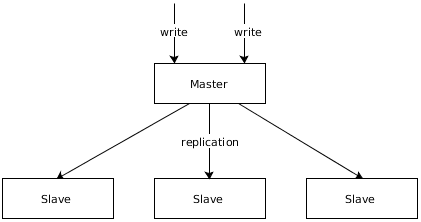
\includegraphics[width=.6\textwidth]{img/replication-master-slave.png}
  \caption{Master-slave replication}
  \label{img:replication-master-slave}
\end{figure}

Another important feature related to the architecture of a storage cluster is the replication model and capabilities.
Replication models are characterised and divided based upon the amount of \textit{masters} and \textit{slaves} in the cluster.
A \textit{master} is a server that is the authoritative source for data, while a \textit{slave} is a node that is dependent on the master for certain queries.
This implies that in a master-slave replicated cluster, all write requests go solely to the master node, which then replicates the modifications to the slave nodes.
While master nodes can handle read and write requests, slave nodes can only handle read requests.
The inherent scalability for read requests in this architecture means it is a very good candidate for data models where the read requests outnumber the write requests by a large amount.

As a side-effect, the cluster itself is more resilient to slave node failures: when a slave node goes down, the remaining nodes can balance the load and the cluster can continue to function.
However, a master failure in this setup renders the cluster at least read-only, and -- depending on the sharding configuration -- potentially only able to serve part of the data that was stored on the nodes.
Neo4j is an example of a data store that operates under a master-slave replication configuration.
% TODO: references
In certain cases the cluster is able to automatically recover from a master failure by a process called \textit{master election}, where a new authoritative master node is chosen.
This type of capability is commonly seen by data stores supporting more simple data models, such as key-value stores.

\begin{figure}
  \centering
  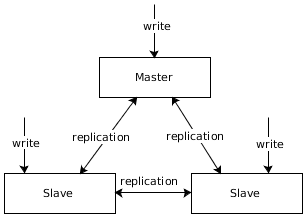
\includegraphics[width=.4\textwidth]{img/replication-master-master.png}
  \caption{Master-master replication}
  \label{img:replication-master-master}
\end{figure}

% TODO: fact check
Similarly to Neo4j, MongoDB operates in a master-slave configuration: one authoritative master, and an undetermined amount of slave nodes.
CouchDB on the contrary, supports a multi-master or master-to-master configuration.
These configurations allow for multiple master nodes to exist within the cluster, and CouchDB implements a quorum algorithm between master nodes in order to allow for eventual consistency in the cluster.
% TODO: use cases for multi-master/master-master

% TODO: reference to some paper about rdbms locking
Finally, the way a data store implements its concurrency control algorithm is important for both horizontal and vertical scalability.
Traditionally, relational database management systems handle concurrent accesses using a pessimistic locking system, utilizing row-, table- and database-level locks.
Two type of locks exist in this context: \TODO{mutual} locks (colloquially known as \texit{reader locks}), and exclusive locks (\textit{writer locks}).
The former implements a mechanism to allow an undetermined amount of requests to access the data without mutating it, the latter prevents more than one request to modify the data at the same time, provided there are no existing reader or writer locks.

In this aspect, Neo4j behaves more like a relational database.
As mentioned before, all write requests are handled by the master node in the cluster, and the concurrent requests are restricted using a lock mechanism.

% TODO: fact check
CouchDB takes an entirely different approach to concurrency control.
Revision control is a feature built natively into the data store, and it is used in a mechanism called Multi-Version Concurrency Control (MVCC) to provide concurrent write access to data.
In short, MVCC redirects running write requests on a document to a new version of that document, while still serving the old version to concurrent read requests.
Once the write request on the new version is finished, the pointer pointing to the most recent version of the document is updated to point to the new, updated document instead of the old, obsolete document.
This also has the benefit of automatically making document writes atomic, since only one value has to be updated in the end: the document pointer.
% TODO: conflict resolution?

MongoDB also makes use of MVCC, however certain requests are still restricted using locks.
This relates to requests that modify the entire database management system, the database or the collection and \TODO{mutual} and exclusive locks are enforced respectively.

\begin{landscape}
  % TODO: references
\begin{table}
  \sffamily
  \begin{tabular}{l l l l l l l l l}
    \toprule
    &
    &
    \multicolumn{4}{l}{\textbf{Features}}\\

    \cline{3-5}

    &
    &
    \textbf{License} &
    \textbf{Commercial support} &
    \textbf{Cloud environment}\\

    \cline{3-6}

    \multirow{2}{*}{\makecell[l]{\textbf{Document}\\\textbf{stores}}} &
    \textbf{MongoDB} &
    \makecell[l]{GNU AGPLv3 (database)\\Apache (drivers)} &
    % https://www.mongodb.com/commercial-license
    Yes &
    % https://www.mongodb.com/cloud
    \makecell[l]{Amazon EC2\\Google Cloud Platform\\Microsoft Azure\\Digital Ocean\\Cloud hosting partners} & \\

    \cline{2-6}

    &
    \textbf{CouchDB} &
    Apache &
    No &
    No & \\

    \cline{2-6}

    \makecell[l]{\textbf{Graph}\\\textbf{stores}} &
    \textbf{Neo4j} &
    \makecell[l]{GNU GPLv3 (Community Edition),\\AGPLv3 (Enterprise Edition)} &
    % https://neo4j.com/licensing/
    Yes &
    % https://neo4j.com/developer/guide-cloud-deployment/
    \makecell[l]{Amazon EC2\\Google Cloud Platform\\Microsoft Azure\\Digital Ocean\\Cloud hosting partners} & \\

    \bottomrule
  \end{tabular}

  \caption{NoSQL data stores: Hosting concerns}
  \label{tbl:hosting}
\end{table}

\end{landscape}

Table \ref{tbl:hosting} provides insight into the aspects related to hosting one or more database instances.
First, the type of license is important when hosting the data store.
Since we have restricted our research to licenses classified as free by the \textcite{FreeSoftwareFoundation1985}, none of these data stores prevent hosting instances without incurring additional licensing costs.
However, for two out of three data stores commercial support is available as well.
Commercial support includes licensing the product for enterprise use, which usually includes additional functionality -- commonly related to scalability -- and customer support.

MongoDB is dual-licensed.
% https://www.gnu.org/licenses/agpl-3.0.en.html
% https://www.apache.org/licenses/LICENSE-2.0
The database management system itself is licensed under the GNU Affero General Public License version 3.
The language bindings -- called drivers -- while officially supported are licensed under a different license, the Apache license

% https://www.gnu.org/licenses/why-affero-gpl.en.html
The GNU Affero General Public License version 3 is a modified version of the GNU General Public License version 3.
The GNU General Public License requires developers that modify software licensed under the GPL to distribute their modifications as well.
However, the license does not cover the case of service providers: if a developer modifies the source code and runs the software on a server, allowing other users to interact with it, distribution of the modified source code is not required.
The AGPL adds a provision to prevent this loophole.
Whenever a modified version of software licensed under the AGPL runs on a server, the modified source code must be available to download.
In the case of data stores, this makes sure that the software remains free and cannot be commercially exploited.

CouchDB, being an Apache project, is licensed under the Apache license.

The Neo4j graph store is dual-licensed as well: the Community Edition is licensed under the GPL version 3, and the Enterprise edition is licensed under the AGPL version 3.\\
Deciding on data store hosting is a difficult topic, which is not within the scope of this research.
We merely enumerate the options available for every data store.
Since all products are licensed under a free license, it is possible for invididuals and companies to host instances themselves.
MongoDB and Neo4j provide commercial support for this use case.
However, running a data store instance can also be outsourced to a plethora of companies and hosting providers.
Both MongoDB and Neo4j integrate with various cloud providers such as Amazon EC2, Google Cloud Platform or the Digital Ocean hosting platform.\\

%% Conclusion
